\section{Experimental Evaluation}
\label{sec:results}

We now present and discuss experimental results from our evaluation of
our system. First, we examine the effectiveness of our security
schemes as implemented in SecondWrite on a set of security benchmarks
previously proposed by Wilander and Kamkar~\cite{wilander2003} for
evaluating the effectiveness of buffer overflow defenses. Second, we
examine how effective our scheme is in protecting against real-world
attacks on widely-used real code (not benchmarks). Third, we examine
the overheads of both the binary rewriter and our security scheme on
some SPEC2006 and other benchmarks.

\mypar{Synthetic Results} In order to test how effective our scheme
is, we utilized the benchmarks provided by Wilander and Kamkar
\cite{wilander2003}. Twenty buffer overflow attack forms were
developed, in order to evaluate the effectiveness of tools available
at the time that aimed to mitigate buffer overflow attacks. The attack
forms covered every combination of buffer overflow attacks on global,
stack, and heap buffers overflowing to a return addresses, base
pointers, function pointers, and \emph{longjmp} buffers. An attack
form is defined as a combination of a technique, location, and an
attack target. Of the twenty attack forms, we obtained the source code
to only eighteen of these attack forms. We then compiled the programs into binary code which we then rewrote using SecondWrite.
Our schemes in SecondWrite successfully
defended against all attack forms in the Wilander and Kamkar
benchmarks.

\mypar{Real World Attacks} Ultimately, the success of our scheme depends on whether or not attacks that are observed in the real world can be prevented or not. Two real-world attacks were tested.

The first application we tested was a HTTP server named GHTTPD. This web server has a stack buffer overflow vulnerability in its logging function \cite{ghttpd}. We obtained an exploit for this application which overflows a stack-based buffer and corrupts the return address. Using the return address protection component of our scheme, we were able to protect the return address and prevent the attack that uses the buffer overflow vulnerability to  corrupt the return address. When our protection scheme is enabled, the return address corruption is detected when the attack occurs and the application is aborted.

% Padraig: Give a reference to the GHTTPD attack.  Even a website reference is fine.
% DONE

The second application we tested was another HTTP server named CoreHTTP. This application contains a buffer-overflow vulnerability where it fails to adequately check user-supplied data before copying it to an insufficiently sized buffer \cite{corehttp}. We obtained an exploit for this application and applied our protection scheme to the application. Again, when our protection scheme is enabled, the attack is detected and the application is aborted.

\mypar{Binary Rewriting Overhead} A subset of SPEC benchmarks and
other benchmarks were selected to substantiate the performance of our
binary rewriter. The benchmarks were selected at random, and
are limited only by the criteria that they are correctly rewritten by
our still-early prototype. Table~\ref{benchlist} lists the set of
benchmarks that are used in the experiments. All the benchmarks are
compiled with gcc 4.4.1.

% Padraig: This section in two places (here and at the beginning of
% the section talks about "SPEC and other" benchmarks.  It is possible
% that by Friday when Kapil submits his paper all his benchmarks will
% be SPEC, in which case you can use those and take out the "and
% other" phrase.

\begin{table}
\begin{center}
\begin{tabular}{ | c | c | c | }
\hline
\textbf{Application} & \textbf{Source} & \textbf{Lines of C Source Code} \\
\hline
\hline
lbm & SpecFP2006 & 1155 \\
\hline
art & OMP2001 & 1914 \\
\hline
mcf & SpecInt2006 & 2685 \\
\hline
libquantum & SpecInt2006 & 4357 \\
\hline
sjeng & SpecInt2006 & 13847 \\
\hline
hmmer & SpecInt2006 & 35992 \\
\hline
h264 & SpecInt2006 & 51578 \\
\hline
\end{tabular}
\end{center}

\caption{Application Characteristics}
\label{benchlist}
\end{table}

In the first experiment, all binaries executed correctly after
rewriting thereby demonstrating the robustness of our binary
rewriter. We were able to correctly apply the standard suite of LLVM
optimization passes without any changes. These include CFG
simplification, global optimization, global dead-code elimination,
inter-procedural constant propagation, instruction combining,
condition propagation, tail-call elimination, induction variable
simplification and selective loop unrolling.

Besides correctness, the next most important metrics are the run-time
speedup or overhead of the rewritten binaries versus the input
binaries. For this paper, we study the performance of our rewriter on
already optimized binaries. Figure \ref{withopts} shows the normalized
execution time of each rewritten binary compared to an input binary
produced using GCC with the highest available level of optimization
(-O3 flag). The results are mixed, with most benchmarks
nearly breaking even or showing a small slowdown, one benchmark
showing a larger slowdown of 20\%, and one benchmark actually shows a
speedup of 16\%. The average is 3\% slowdown.\footnote{Rewriting unoptimized input binaries produced using GCC -O0 yields an average speedup of 27\% using SecondWrite (not shown) due to its optimizations.}

\begin{figure}[ht!]
\begin{center}
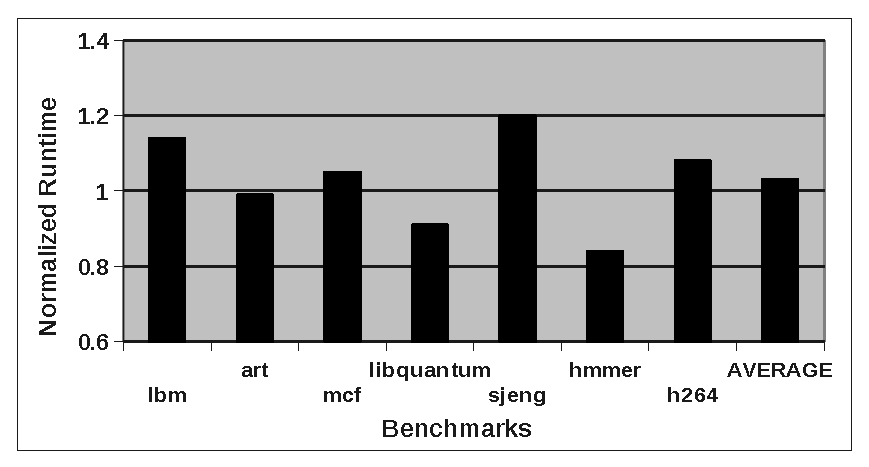
\epsfig{file=images/perfopt4.eps}
\par\end{center}
%\renewcommand{\baselinestretch}{1}
%\small\normalsize
%\begin{quote}
\vspace{-.2in}
\caption{Normalized runtime of rewritten binary as compared to optimized input
  binary (runtime=1.0).}
\label{withopts}
%\end{quote}
\end{figure}
%renewcommand{\baselinestretch}{2}

We consider this near break-even performance on highly optimized
binaries a good result for the following three reasons:

\mybeginlist

\item Our initial goal was not necessarily to get a speedup, but to
  generate correct IR without without introducing too much
  overhead. This would enable the IR to be a starting point for
  various custom compiler transformations we wanted to perform
  thereafter, such as automatic parallelization or security as covered
  in this thesis. Ultimately, these optimizations determine the
  utility of the rewriter.

\item These numbers represent our first-cut implementation devoid of
  any attempt at producing a better IR more geared towards
  optimization. We believe these numbers can be substantially improved
  with more detailed IR and are exploring several related avenues.

\item We have currently not implemented any custom serial
  optimizations that might improve performance further, such as the
  inter-procedural versions of common sub-expression elimination and
  loop-invariant code motion, changing the compiler-enforced calling
  convention for registers for better run-time, and more aggressive
  inlining. We believe these optimizations hold promise as the
  inter-procedural optimization abilities of current compilers are
  very limited compared to their intra-procedural performance.

\end{list}

One additional advantage of the binary rewriter is that it accumulates
optimizations across two compilers---rewritten binaries have an
optimization if it is either present in the compiler that produced the
input binary, or in the rewriter. In our case, if either GCC or LLVM
had an optimization, the output binary should have it. This is why,
for example, one of our rewritten binaries (\emph{hmmer}) had a 16\%
speedup versus the input binary. Although GCC with the -O3
optimization flag is known to produce good code, in some cases it
missed promoting structure fields to registers whereas LLVM did,
explaining the speedup in \emph{hmmer}. With better IR and more
aggressive optimizations, we expect to see more consistent speedups in
output binaries in the future.

\mypar{Security Related Overheads} The overhead of the security
schemes was measured on the same applications as used for
measuring the overhead of the binary rewriter. The results are presented in Figure \ref{fig:security} and show overhead versus rewritten binaries without security schemes inserted. As seen, the average run-time overhead of 7\% introduced by the protection scheme is low.

\begin{figure}[ht!]
\begin{center}
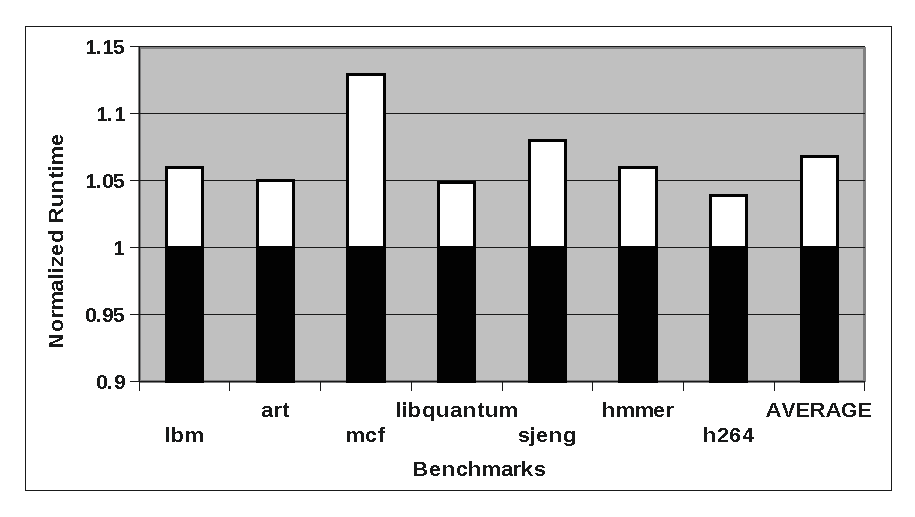
\epsfig{file=images/sec.eps}
\end{center}
%%\renewcommand{\baselinestretch}{1}
%%\small\normalsize
%%\begin{quote}
\vspace{-.2in}
\caption{Normalized runtime of rewritten binary with security scheme added.}
\label{fig:security}
%%\end{quote}
\end{figure}
%%\renewcommand{\baselinestretch}{2}

%Next, we measured the overheads of adding the protection scheme to the applications we used for our real-world experiments. These results are presented in Figure .
